\section{\CEU}
\label{sec.ceu}

\CEU is a synchronous reactive language in which programs advance in a sequence
of discrete reactions to external events.
%
It is designed for control-intensive applications, supporting concurrent lines
of execution, known as \emph{trails}, and instantaneous broadcast communication
through events.
%
Computations within a reaction (such as expressions, assignments, and
system calls) are also instantaneous in accordance to the synchronous
hypothesis~\cite{rp.hypothesis}.
%
\CEU provides an \code{await} statement which is the only that actually
``consumes'' time.
%
An \code{await} statement blocks the current running trail allowing the program
to advance its other trails; when all trails are blocked, the reaction
terminates and control returns to the environment.

In \CEU, every execution path within loops must contain at least one
\code{await} statement~\cite{ceu.sensys13,esterel.primer}.
%
This restriction, which is statically checked by the compiler, ensures that
every reaction runs in bounded time, eventually terminating with all trails
blocked in \code{await} statements.
%
\CEU has an additional restriction, which it shares with Esterel and
synchronous languages in general~\cite{esterel.preemption}: computations that
take a non-negligible time to run (e.g., cryptography or image processing
algorithms) violate the zero-delay hypothesis, and thus cannot be directly
implemented.

Listing~\ref{lst.syntax} shows a compact reference of~\CEU:

\bgroup
\def\T<#1>{\langle\mathit{#1}\rangle}
\def\C#1#2{\hfill\rmfamily\itshape\makebox[#1\columnwidth][l]{//~#2}}
\begin{lstlisting}[
  basicstyle=\ttfamily\footnotesize,
  caption={The concrete syntax of \CEU.},
  label={lst.syntax},
]
|\C{1.}{Declarations}|
input $\T<type>$ $\T<id>$; | \C{.6}{declares external input event} |
event $\T<type>$ $\T<id>$; | \C{.6}{declares internal event}       |
var   $\T<type>$ $\T<id>$; | \C{.6}{declares variable}             |

|\C{1.}{Event handling}|
$\T<id>$ = await $\T<id>$;   | \C{.6}{awaits event and assigns received value} |
$\T<id>$ = await $\T<time>$; | \C{.6}{awaits time and assigns delayed delta}   |
emit $\T<id>$($\T<exp>$);    | \C{.6}{emits event passing value}               |

|\C{1.}{Control flow}|
$\T<stmt>$ ; $\T<stmt>$                       | \C{.45}{sequence}     |
if $\T<exp>$ then $\T<stmts>$ else $\T<stmts>$ end | \C{.45}{conditional}  |
loop do $\T<stmts>$ end                   | \C{.45}{repetition}   |
finalize [$\T<stmts>$] with $\T<stmts>$ end    | \C{.45}{finalization} |

|\C{1.}{Logical parallelism}|
par/or  do $\T<stmts>$ with $\T<stmts>$ end | \C{.45}{aborts when any side ends}      |
par/and do $\T<stmts>$ with $\T<stmts>$ end | \C{.45}{terminates when all sides ends} |
par     do $\T<stmts>$ with $\T<stmts>$ end | \C{.45}{never terminates}               |

|\C{1.}{Assignment \& Integration with C}|
$\T<id>$ = $\T<exp>$; | \C{.6}{assigns value to variable}                |
_$\T<id>$($\T<exps>$) | \C{.6}{calls C function (id starts with `\_'\,)} |
\end{lstlisting}
\egroup

Listing~\ref{lst.ceu} shows a complete example in \CEU that blinks a LED with a
frequency of 1 second, terminating with a button press always with the LED off.
%
The implementation first declares the \code{BUTTON} as an input event (ln.~1).
Then, it uses a \code{par/or} composition to run two activities in parallel:
a single statement that waits for a button press before terminating (ln.~3),
and an endless loop that blinks the LED on and off (ln.~8--13).
The \code{finalize} clause (ln.~5--7) ensures that, no matter how its enclosing
trail terminates, the LED will be unconditionally turned off (ln.~6).

The \code{par/or} composition, which stands for a \emph{parallel-or}, provides
an orthogonal abortion mechanism in which its composed trails do not know when
and how they are aborted (i.e., abortion is external to them).
%
This is possible to do safely in synchronous languages due to the accurate
control of concurrent activities, i.e., in between every reaction, the whole
system is idle and consistent~\cite{esterel.preemption}.
%
The finalization mechanism extends orthogonal abortion to also work with
activities that use stateful resources from the environment (such as files and
network handlers), as we discuss in Section~\ref{sec.ceu.fin}.
%
\fs{First-class timers.}

\begin{lstlisting}[
  numbers=left,
  basicstyle=\ttfamily\footnotesize,
  float=h,
  caption={A program in \CEU that blinks a LED every second, terminating on a
           button press in a consistent state.},
  label={lst.ceu},
]
input void BUTTON;
par/or do
    await BUTTON;
with
    finalize with
        _led(0);
    end
    loop do
        _led(1);
        await 1s;
        _led(0);
        await 1s;
    end
end
\end{lstlisting}

In \CEU, any identifier prefixed with an underscore (e.g., \code{_led}) is
passed unchanged to the underlying~C compiler.
%
Therefore, access to~C is straightforward and syntactically traceable.
%
To ensure that programs operate under the synchronous hypothesis, the compiler
environment should only provide access to~C operations that can be assumed to
be instantaneous, such as non-blocking~I/O and simple accesses to data
structures.

\subsection{External and Internal Events}
\label{sec.ceu.evts}

\CEU defines time as a discrete sequence of reactions to unique external
input events.
%
External input events are received from the environment, and each delimits a
new logical unit of time that triggers an associated reaction.
%
The life-cycle of a program in \CEU can be summarized as
follows~\cite{ceu.sensys13}:
%
\begin{enumerate}[i]
\item The program initiates a ``boot reaction'' in a single trail (parallel
      constructs may create new trails).
\item Active trails execute until they await or terminate, one after
      another.  This step is called a \emph{reaction chain}, and always runs in
      bounded time.
\item When all trails are blocked, the program goes idle and the environment
      takes control.
\item On the occurrence of a new external input event, the environment
      awakes \emph{all} trails awaiting that event, and the program goes back to
      step~(i).
\end{enumerate}

A program must react to an event completely before handling the next one.
%
By the synchronous hypothesis, the time the program spends in step~(ii) is
conceptually zero (in practice, negligible).
%
Hence, from the point of view of the environment, the program is always
idle on step~(iii).
%
In practice, if a new external input event occurs while a reaction executes,
the event is saved on a queue, which effectively schedules it to be processed
in a subsequent reaction.

\subsubsection*{External events and discrete time}

\begin{figure}[b]
\centering
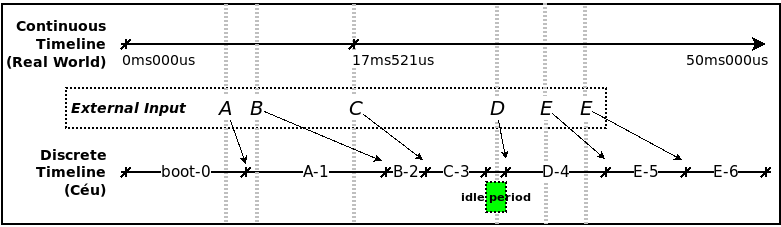
\includegraphics[width=\columnwidth]{tick}
\caption{The discrete notion of time in \CEU.}
\label{fig.ticks}
\end{figure}

The sequential processing of external input events induces a discrete notion of
time in \CEU, as illustrated in Figure~\ref{fig.ticks}.
%
The continuous timeline shows an absolute reference clock with ``physical
timestamps'' for the event occurrences (e.g., event~\code{C} occurs at
$17ms521us$).
%
The discrete timeline shows how the same occurring events fit in the logical
notion of time of \CEU.
%
The boot reaction \code{boot-0} happens before any input, at program startup.
%
Event~\code{A} ``physically'' occurs during \code{boot-0} but, because time
is discrete, its corresponding reaction only executes afterwards, at logical
instant~\code{A-1}.
%
Similarly, event~\code{B} occurs during~\code{A-1} and its reaction is
postponed to execute at~\code{B-2}.
%
Event~\code{C} also occurs during~\code{A-1} but its reaction must also wait
for~\code{B-2} to execute and so it is postponed to execute at~\code{C-3}.
%
Event~\code{D} occurs during an idle period and can start immediately at
\code{D-4}.
%
Finally, two instances of event~\code{E} occur during~\code{D-4}; they are
handled in the subsequent reactions~\code{E-5} and~\code{E-6}.

Unique input events imply mutually exclusive reactions, which execute
atomically and never overlap.
%
Automatic mutual exclusion is a prerequisite for deterministic reactions as
we discuss in Section~\ref{sec.sem}.
%
%8<- - - - - - - - - - - - - - - - - - - - - - - - - - - - - - - - - - - - -
% \gl{A não ser que seja desenvolvido (e.g., explicado e comparado com
%   Esterel) eu acho que o parágrafo anterior é dispensável.}
% \fs{Tirei o "simplifies resoning about concurrency".
%     O resto do parágrafo é absoluto e tenta dar a intuição das condições para
%     ter determinismo.}
%- - - - - - - - - - - - - - - - - - - - - - - - - - - - - - - - - - - - ->8

In practice, the synchronous hypothesis for \CEU holds if reactions execute
faster than the rate of incoming input events.
%
Otherwise, the program would continuously accumulate delays between physical
occurrences and actual reactions for the input events.
%
In the soft real-time systems targeted by \CEU (e.g., sensor networks,
multimedia systems, interactive games, etc.) such delay and postponed
reactions might be tolerated by users as long as they are infrequent and the
application does not take too long to catch up with real time.
%
Note that the synchronous semantics is the norm in typical event-driven
systems, such as event dispatching in UI toolkits, game loops in game engines,
and clock ticks in embedded systems.

\subsubsection*{Internal events as subroutines}

In \CEU, the queue-based processing of events described previously applies
only to external input events, i.e., those events submitted to the program
by the environment.
%
Internal events, which are those events generated internally by the program
via \code{emit} statements, are processed in a stack-based manner.
%
These internal events provide a fine-grained execution control and, because
of their stack-based processing, can be used to implement a limited form of
subroutine, as illustrated in Listing~\ref{lst.sub} below.

\begin{lstlisting}[
  numbers=left,
  basicstyle=\ttfamily\footnotesize,
  float=h,
  caption={A \CEU program with a ``subroutine''.},
  label={lst.sub},
]
event int* inc;     // subroutine |`|inc|'|
par/or do
    loop do         // definitions are loops
        var int* p = await inc;
        *p = *p + 1;
    end
with
    var int v = 1;
    $\cdots$
    emit inc(&v);   // call |`|inc|'|
    _assert(v==2);  // after return
end
\end{lstlisting}
\vskip-\baselineskip

In Listing~\ref{lst.sub}, the ``subroutine'' \code{inc} is defined as a loop
(ln.~3--6) that continuously awaits its identifying event (ln.~4), and
increments the value passed to it by reference (ln.~5).
%
A trail in parallel (ln.~8--11) invokes the subroutine through an \code{emit}
statement (ln.~10).
%
Given the stack-based execution mode of internal events, as the emit executes,
the calling trail pauses, the subroutine awakes (ln.~4), runs its body
(yielding \code{v=2}), loops, and awaits the next ``call'' (ln.~4, again).
%
Only after this sequence does the calling trail resumes and moves on to
execute the assertion (ln.~11).

\CEU also supports nested \code{emit} invocations for internal events.
%
For instance, the body of the subroutine \code{inc} in Listing~\ref{lst.sub}
could \code{emit} another internal event after awaking (ln.~4), creating a
new level in the stack.
%
We can think of the stack as a record of the nested, fine-grained internal
reactions that happen inside the same bigger reaction to some external
event.

This form of subroutine has a significant limitation though: it cannot
express recursion (an \code{emit} to itself is always ignored as a running
trail cannot be waiting on itself).
%
That said, it is this very limitation that brings important safety
properties to subroutines.
%
First, such subroutines are guaranteed to react in bounded time.
%
Second, memory for locals is also bounded, not requiring data stacks.
%
Third, \CEU subroutines can be safely used by the other primitives of the
language, such as parallel compositions and the \code{await} statement,
without breaking the programming model.
%
In particular, after calling a subroutine these primitives wait while
keeping context information, such as locals and the program counter, which
makes the calls behave similarly to those of
coroutines~\cite{lua.coroutines}.
%
Finally, in previous work, we built other advanced control mechanisms on top
of internal events, such as resumable exceptions and reactive
variables~\cite{ceu.rem13}.
%
%In Section~\ref{sec.adv.excpt} we show how to use them to implement
%exceptions.
%
%8<- - - - - - - - - - - - - - - - - - - - - - - - - - - - - - - - - - - - -
\gl{Revisei do início da Seção~2 até aqui.}
%- - - - - - - - - - - - - - - - - - - - - - - - - - - - - - - - - - - - ->8

\subsection{Shared-Memory Concurrency}
    - referenciar warnings

Embedded applications make extensive use of global memory and shared resources,
such as through memory-mapped registers and system calls to device drivers.
Hence, an important goal of \CEU is to ensure a reliable behavior for programs
with concurrent lines of execution sharing memory and interacting with the
environment.

\begin{figure}[h]
\begin{minipage}[h]{0.45\linewidth}
\begin{lstlisting}[numbers=left,xleftmargin=3em]
input void A;
input void B;
var int x = 1;
par/and do
    await A;
    x = x + 1;
with
    await B;
    x = x * 2;
end
\end{lstlisting}
\centering\small{\ax Accesses to \code{x} are never concurrent.}
\end{minipage}
%
\begin{minipage}[h]{0.45\linewidth}
\begin{lstlisting}[numbers=left,xleftmargin=3em]
input void A;
var int y = 1;
par/and do
    await A;
    y = y + 1;
with
    await A;
    y = y * 2;
end
\end{lstlisting}
\centering\small{\bx Accesses to \code{y} are concurrent but deterministic.}
\end{minipage}
%\rule{8.4cm}{0.37pt}
\caption{ Shared-memory concurrency in \CEU:
example \ax is safe because the trails access \code{x} atomically in different
reactions;
example \bx is unsafe because both trails access \code{y} in the same reaction.
\label{lst.shared}
}
\end{figure}

In \CEU, when multiple trails are active during the same reaction, they are
scheduled in lexical order, i.e., in the order they appear in the program
source code.
%
For instance, consider the two examples in Figure~\ref{lst.shared}, both
defining a shared variable (ln. 2), and assigning to it in parallel trails (ln.
5, 8).

In the example \ax, the two assignments to \code{x} can only execute in
reactions to different events \code{A} and \code{B}, which cannot occur
simultaneously by definition (Section~\ref{sec.ceu.evts}).
Hence, for the sequence of events \code{A->B}, \code{x} becomes \code{4}
(\code{(1+1)*2}), while for \code{B->A}, \code{x} becomes \code{3}
(\code{(1*2)+1}).

In the example \bx, the two assignments to \code{y} are simultaneous because
they execute in reaction to the same event \code{A}.
Since \CEU employs lexical order for intra-reaction statements, the execution
is still deterministic, and \code{y} always becomes \code{4} (\code{(1+1)*2}).
%
However, that an (apparently innocuous) change in the order of trails modifies
the behavior of the program.
%
To mitigate this threat, \CEU performs concurrency checks at compile time to
detect conflicting accesses to shared variables:
if a variable is written in a trail segment, then a concurrent trail segment
cannot read or write to that variable~\cite{ceu.sensys13}.
%
Nonetheless, the static checks are optional and do not affect the semantics of
the language.

\subsection{Abortion and Finalization}
\label{sec.ceu.fin}

The \code{par/or} of \CEU is an \emph{orthogonal abortion
mechanism}~\cite{esterel.preemption} because the two sides in the composition
need not be tweaked with synchronization primitives or state variables in order
to affect each other.
%
In addition, abortion is \emph{immediate} in the sense that it executes
atomically in the current micro reaction.
%
Immediate orthogonal abortion is a distinctive feature of synchronous languages
and cannot be expressed effectively in traditional (asynchronous)
multi-threaded languages~\cite{esterel.preemption,sync_async.threadsstop}.

However, aborting lines of execution that deal with external resources may lead
to inconsistencies.
%
For this reason, \CEU provides a \code{finalize} construct to unconditionally
execute a series of statements even if the enclosing block is aborted.

\CEU also enforces the use of \code{finalize} for system calls that deal with
pointers representing resources, as illustrated in the two examples of
Figure~\ref{lst.fin.ceu}:
%
\begin{itemize}
\item If \CEU \textbf{passes} a pointer to a system call (ln. \ax:5), the
pointer represents a \textbf{local} resource (ln. \ax:2) that requires finalization
(ln. \ax:7).
\item If \CEU \textbf{receives} a pointer from a system call return (ln. \bx:4),
the pointer represents an \textbf{external} resource (ln. \bx:2) that requires
finalization (ln. \bx:6).
\end{itemize}
%
\CEU tracks the interaction of system calls with pointers and requires
finalization clauses to accompany them.
%
In the example in Figure~\ref{lst.fin.ceu}.a, the local variable \code{msg}
(ln. 2) is an internal resource passed as a pointer to \code{\_send\_request}
(ln. 5), which is an asynchronous call that transmits the buffer in the
background.
If the block aborts (ln. 11) before receiving an acknowledge from the
environment (ln. 9), the local \code{msg} goes out of scope and the external
transmission now holds a \emph{dangling pointer}.
The finalization ensures that the transmission also aborts (ln. 7).
%
In the example in Figure~\ref{lst.fin.ceu}.b, the call to \code{\_fopen} (ln.
4) returns an external file resource as a pointer.
If the block aborts (ln. 12) during the \code{await A} (ln. 9), the file
remains open as a \emph{memory leak}.
The finalization ensures that the file closes properly (ln. 6).
%
In both cases, the code does not compile without the \code{finalize}
construct.%
\footnote{
The compiler only forces the programmer to write the finalization clause, but
cannot check if it actually handles the resource properly.
}

The finalization mechanism of \CEU is fundamental to preserve the orthogonality
of the \code{par/or} construct since the clean up code is encapsulated in the
aborted trail itself.

\begin{figure}
\begin{minipage}[t]{0.48\linewidth}
\begin{lstlisting}[numbers=left,xleftmargin=3.5em,mathescape=true]
par/or do
   var _buffer_t msg;
   <...> // prepare msg
   finalize
      _send_request(&msg);
   with
      _send_cancel(&msg);
   end
   await SEND_ACK;
with
   <...>
end
.
\end{lstlisting}
\centering\small{\ax Local resource finalization}
\end{minipage}
%
\begin{minipage}[t]{0.48\linewidth}
\begin{lstlisting}[numbers=left,xleftmargin=3.5em]
par/or do
   var _FILE* f;
   finalize
      f = _fopen(...);
   with
      _fclose(f);
   end
   _fwrite(..., f);
   await A;
   _fwrite(..., f);
with
   <...>
end
\end{lstlisting}
\centering\small{\bx External resource finalization}
\end{minipage}
%\rule{8.4cm}{0.37pt}
\caption{
\CEU enforces the use of finalization to prevent \emph{dangling pointers} for
local resources and \emph{memory leaks} for external resources.
\label{lst.fin.ceu}
}
\end{figure}
